\documentclass[runningheads,a4paper]{llncs}
\usepackage{amssymb}
\usepackage{url}
\usepackage{times}
\usepackage{float}
\usepackage[T1]{fontenc}
\usepackage{graphicx}
\usepackage{color}
\usepackage{soul}  
\usepackage{nameref}  
\usepackage{amsbsy}  
\usepackage{bezier}  
\usepackage{colortbl}  
\usepackage[leqno,fleqn]{amsmath}  
\usepackage{verbatim}
\usepackage{listings}
\usepackage[utf8]{inputenc}


\setcounter{tocdepth}{3}
\newcommand{\keywords}[1]{\par\addvspace\baselineskip
\noindent\keywordname\enspace\ignorespaces#1}

\begin{document}
\mainmatter

\title{Title of Your Research Report}
\subtitle{A Paper Study Report}
\date{Spring Semester 2018}

\author{John Doe}

\institute{
Boston University\\ Metropolitan College \\ Department of Computer Science  \\
\{john.due\}@bu.edu \\
\url{http://www.bu.edu/metcs}
}

\maketitle



\begin{abstract}
The abstract should summarize the contents of the paper and should
contain at least 70 and at most 150 words. It should be written using the
\emph{abstract} environment.
\keywords{We would like to encourage you to list your keywords within
the abstract section}
\end{abstract}


% add your own Keywords. 
\keywords{Big Data Analysis, Cloud Computoing}

\section{Introduction}

You are strongly encouraged to use \LaTeXe{} for the
preparation of your camera-ready manuscript together with the
corresponding Springer class file \verb+llncs.cls+. Only if you use
\LaTeXe{} can hyperlinks be generated in the online version
of your manuscript.

The \LaTeX{} source of this instruction file for \LaTeX{} users may be
used as a template. This is
located in the ``authors'' subdirectory in
\url{ftp://ftp.springer.de/pub/tex/latex/llncs/latex2e/instruct/} and
entitled \texttt{typeinst.tex}. There is a separate package for Word 
users. Kindly send the final and checked source
and PDF files of your paper to the Contact Volume Editor. This is
usually one of the organizers of the conference. You should make sure
that the \LaTeX{} and the PDF files are identical and correct and that
only one version of your paper is sent. It is not possible to update
files at a later stage. Please note that we do not need the printed
paper.

We would like to draw your attention to the fact that it is not possible
to modify a paper in any way, once it has been published. This applies
to both the printed book and the online version of the publication.
Every detail, including the order of the names of the authors, should
be checked before the paper is sent to the Volume Editors.

\subsection{This is subsection example}

SOME Example text here ... 

Kindly assure that the Contact Volume Editor is given the name and email
address of the contact author for your paper. The Contact Volume Editor
uses these details to compile a list for our production department at
SPS in India. Once the files have been worked upon, SPS sends a copy of
the final pdf of each paper to its contact author. The contact author is
asked to check through the final pdf to make sure that no errors have
crept in during the transfer or preparation of the files. This should
not be seen as an opportunity to update or copyedit the papers, which is
not possible due to time constraints. Only errors introduced during the
preparation of the files will be corrected.

This round of checking takes place about two weeks after the files have
been sent to the Editorial by the Contact Volume Editor, i.e., roughly
seven weeks before the start of the conference for conference
proceedings, or seven weeks before the volume leaves the printer's, for
post-proceedings. If SPS does not receive a reply from a particular
contact author, within the timeframe given, then it is presumed that the
author has found no errors in the paper. The tight publication schedule
of LNCS does not allow SPS to send reminders or search for alternative
email addresses on the Internet.

In some cases, it is the Contact Volume Editor that checks all the final
pdfs. In such cases, the authors are not involved in the checking phase.

\subsection{Additional Information Required by the Volume Editor}

If you have more than one surname, please make sure that the Volume Editor
knows how you are to be listed in the author index.


\subsection{Figures}

For \LaTeX\ users, we recommend using the \emph{graphics} or \emph{graphicx}
package and the includegraphics command.

Please check that the lines in line drawings are not
interrupted and are of a constant width. Grids and details within the
figures must be clearly legible and may not be written one on top of
the other. Line drawings should have a resolution of at least 800 dpi
(preferably 1200 dpi). The lettering in figures should have a height of
2~mm (10-point type). Figures should be numbered and should have a
caption which should always be positioned \emph{under} the figures, in
contrast to the caption belonging to a table, which should always appear
\emph{above} the table; this is simply achieved as matter of sequence in
your source.

Please center the figures or your tabular material by using the \verb+\centering+
declaration. Short captions are centered by default between the margins
and typeset in 9-point type (Fig.~\ref{fig:example} shows an example).
The distance between text and figure is preset to be about 8~mm, the
distance between figure and caption about 6~mm.

To ensure that the reproduction of your illustrations is of a reasonable
quality, we advise against the use of shading. The contrast should be as
pronounced as possible.

If screenshots are necessary, please make sure that you are happy with
the print quality before you send the files.


\begin{figure}
\centering
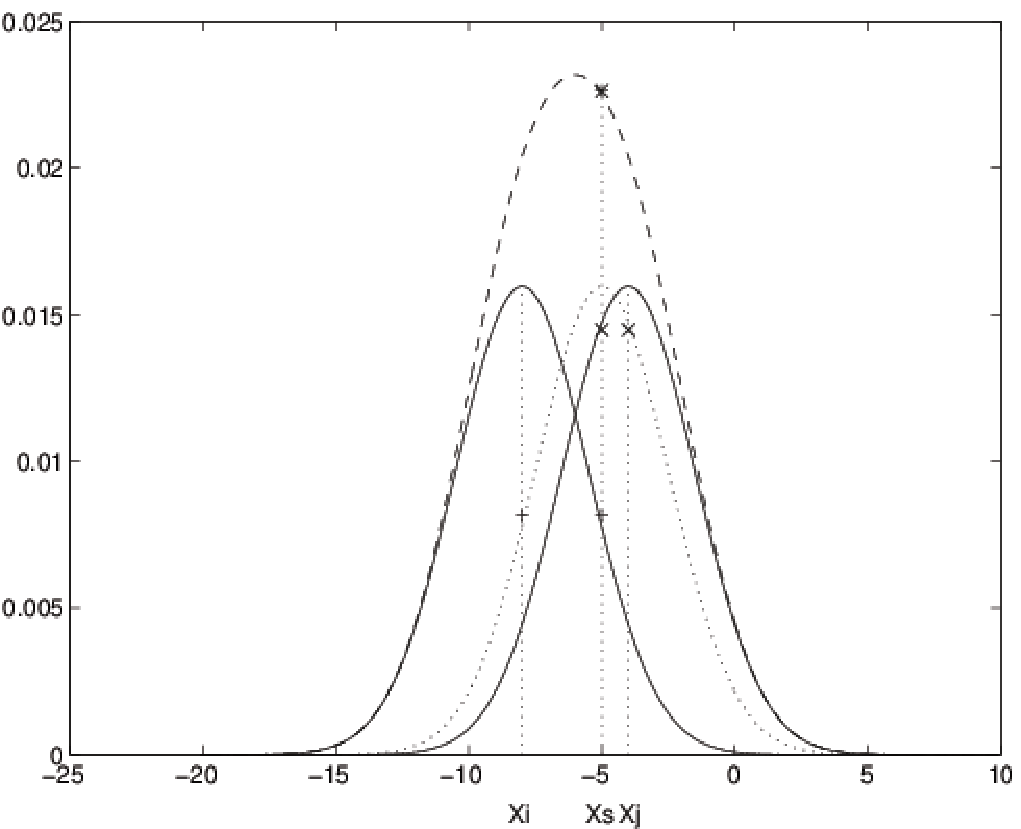
\includegraphics[height=6.2cm]{images/eijkel2}
\caption{One kernel at $x_s$ (\emph{dotted kernel}) or two kernels at
$x_i$ and $x_j$ (\textit{left and right}) lead to the same summed estimate
 at $x_s$. This shows a figure consisting of different types of
 lines. Elements of the figure described in the caption should be set in
 italics, in parentheses, as shown in this sample caption.}
 \label{fig:example}
 \end{figure}



Please define figures (and tables) as floating objects. Please avoid
using optional location parameters like ``\verb+[h]+" for ``here".

\paragraph{Remark 1.}

In the printed volumes, illustrations are generally black and white
(halftones), and only in exceptional cases, and if the author is
prepared to cover the extra cost for color reproduction, are colored
pictures accepted. Colored pictures are welcome in the electronic
version free of charge. If you send colored figures that are to be
printed in black and white, please make sure that they really are
legible in black and white. Some colors as well as the contrast of
converted colors show up very poorly when printed in black and white.

\subsection{Formulas}

Displayed equations or formulas are centered and set on a separate
line (with an extra line or halfline space above and below). Displayed
expressions should be numbered for reference. The numbers should be
consecutive within each section or within the contribution,
with numbers enclosed in parentheses and set on the right margin --
which is the default if you use the \emph{equation} environment, e.g.,

\begin{equation}
  \psi (u) = \int_{o}^{T} \left[\frac{1}{2}
  \left(\Lambda_{o}^{-1} u,u\right) + N^{\ast} (-u)\right] dt \;  .
\end{equation}

Equations should be punctuated in the same way as ordinary
text but with a small space before the end punctuation mark.

\subsection{Footnotes}

The superscript numeral used to refer to a footnote appears in the text
either directly after the word to be discussed or -- in relation to a
phrase or a sentence -- following the punctuation sign (comma,
semicolon, or period). Footnotes should appear at the bottom of
the
normal text area, with a line of about 2~cm set
immediately above them.\footnote{The footnote numeral is set flush left
and the text follows with the usual word spacing.}

\subsection{Program Code}

Program listings or program commands in the text are normally set in
typewriter font, e.g., CMTT10 or Courier.

\medskip

\noindent
{\it Example of a Computer Program}
\begin{verbatim}
program Inflation (Output)
  {Assuming annual inflation rates of 7%, 8%, and 10%,...
   years};
   const
     MaxYears = 10;
   var
     Year: 0..MaxYears;
     Factor1, Factor2, Factor3: Real;
   begin
     Year := 0;
     Factor1 := 1.0; Factor2 := 1.0; Factor3 := 1.0;
     WriteLn('Year  7% 8% 10%'); WriteLn;
     repeat
       Year := Year + 1;
       Factor1 := Factor1 * 1.07;
       Factor2 := Factor2 * 1.08;
       Factor3 := Factor3 * 1.10;
       WriteLn(Year:5,Factor1:7:3,Factor2:7:3,Factor3:7:3)
     until Year = MaxYears
end.
\end{verbatim}
%




\section{References and Citations}

For Citations you should use the Bibtext Format. Here is an example text paragraph with citations inside. 

Over time, various efforts were aimed at extending this simple model---most notably object-oriented \cite{atkinson1989object} (or object-relational \cite{stonebraker1995object})
 systems in the 1980's. 

But, no doubt following the slow integration of generic programming into mainstream object-oriented languages (C++ did not offer templates until 1991 \cite{stroustrup1996history} and Java lacked generics until 2004 \cite{parnin2013adoption}), such systems arguably did not offer much in the way of additional functionality compared to the flat relational model, besides pointers and some support for inheritance, and as such, the efforts never gained widespread attraction.


\textbf{Storing Complex Objects.} Today, however, the data management landscape is awash in cloud-based systems supporting many complex data types \cite{white2009hadoop,zaharia2010spark,yu2008dryadlinq,alexandrov2014stratosphere,Melnik:2010:DIA:1920841.1920886,Alsubaiee:2014:ASO:2733085.2733096,chodorow2013mongodb}. 



\bibliographystyle{plain}
% it referes to the file named literature.bib 
\bibliography{literature}  


\end{document}
